\documentclass[11pt]{article}
\usepackage{colacl}
\usepackage{graphicx} %for pic
\usepackage{tabularx}
\usepackage{hyperref}
\hypersetup{
    colorlinks = true,
    linkcolor = {blue},
    citecolor = {blue},
}
\usepackage{caption}
% \usepackage{pbox}
\usepackage{multirow}

\sloppy

\title{Running time experiments between Treap and Dynamic Array}
\author{Pingzhou Li}

\begin{document}
\maketitle

%\begin{abstract}
%This is a \LaTeX\ sample for your paper.
%You shouldn't plan to include an abstract for a paper of this length.
%\end{abstract}

\section{Introduction}

Treap and Dynamic Array are two classical data structure with different features. Multiple experiments will be conducted to compare the performances between two data structures on several types of data sequence.

\section{Experiment environment}
I setup the experiment environment on my laptop which has an Intel i7-6700HQ 8 Cores 2.6Hz CPU and 4x16G DDR4 2400MHz memory.
Programming language is Python 3.9 in Windows 10 operating system.

\section{Data generation}
Every data element is generated with id and key, which are both integers.
Id is a unique identifier started from 1 and will be 1 more for next data element.
Key will be drawn uniformly at random from the range 0 to $10^7$.  
A sequence of operations, which contain search, insert, and delete, will be generated and applied to both data structures.
For insert operation, a data element and an operation symbol (integer 1) will be bound together.
For delete or search, a key and an operation symbol (2 indicates delete or 3 indicates search) will be bounded together.

\section{Experiments}
In all experiments, I will generate a sequence of operations which may contain one or more kinds of operations.
If the sequence is a combination of different types of operations, each type of operation will be generated by a specific probability for each operation.
For example, a sequence of 1,000,000 (use M to denote it later) operations, which has 5\% of search and 5\% of delete, will be generated with each operation by 5\% of search and 5\% of delete and 90\% of insert.
Then run the operations on Treap and Dynamic Array to see the different time-consuming.

\subsection{Experiment 1}
In experiment 1, 5 sequences of insert operations will be generated in length of 0.1M, 0.2M, 0.5M, 0.8M and 1M respectively.
And then input the 5 sequences to treap and to dynamic array.
\begin{figure}
\centering
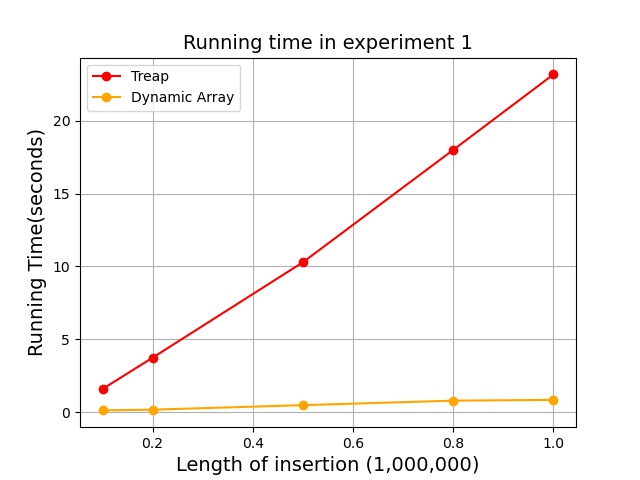
\includegraphics[width=7.5cm]{exp1.jpg} %[pic size]{pic path}
\caption{Running time for different size of insertions}\label{figure1} %pic title
\end{figure}

Figure \ref{figure1} has shown the running time on two data structure. 
The treap spend more time than dynamic array through the whole experiment.
In class, it was shown that treap has a $O(log\ n)$ complexity for insertion whilst dynamic array has a $O(1)$ complexity for insertion.
And in Figure \ref{figure1}, the time spent on dynamic array is quite steady to a constant number.
In contrast, the time spent on treap is going up relatively fast as the number of insertions becomes bigger.

\subsection{Experiment 2}
I generate five 1M long sequences of operations combined insertions and deletions together.
In the sequences, the deletion probabilities are 0.1\%, 0.5\%, 1\%, 5\%, and 10\% for each respectively.

\begin{figure}
\centering
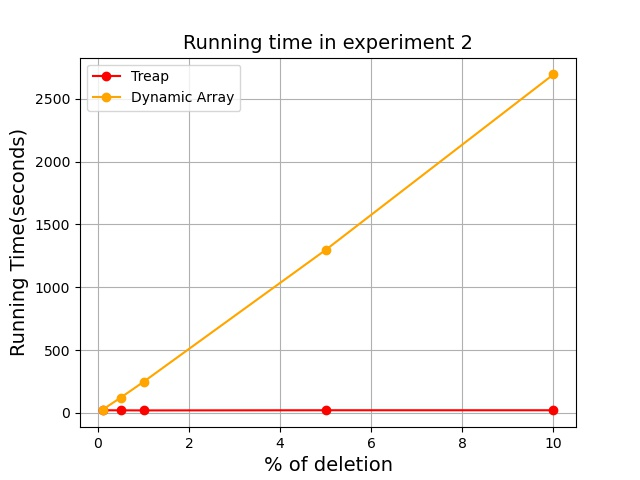
\includegraphics[width=7.5cm]{exp2.jpg} %[pic size]{pic path}
\caption{Running time for different percentage of deletions}\label{figure2} %pic title
\end{figure}

As shown in Figure \ref{figure2}, the treap's time-consuming does not change much while the dynamic array's time-consuming increases in linear.
Insertion of treap has a $O(log\ n)$ complexity and insertion of dynamic array has a $O(n)$ complexity.
As the size of data increases, dynamic array will spend much more time in inserting than treap.

\subsection{Experiment 3}
In comparison to experiment2, I generate five 1M long sequences of operations combined insertions and searches together.
The search probabilities of sequence are 0.1\%, 0.5\%, 1\%, 5\%, and 10\% for each respectively.
  
\begin{figure}
\centering
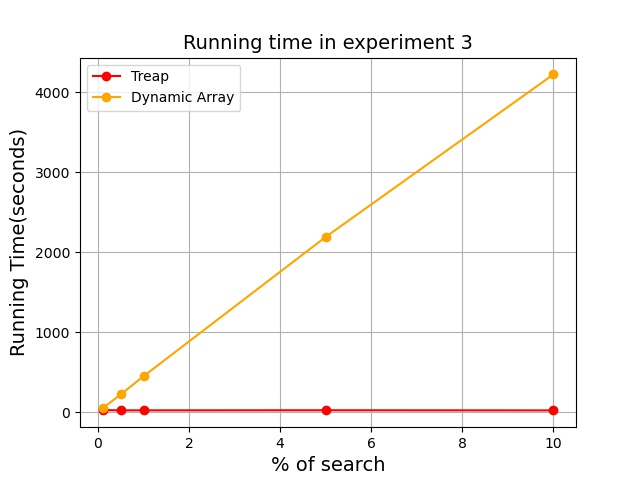
\includegraphics[width=7.5cm]{exp3.jpg} %[pic size]{pic path}
\caption{Running time for different percentage of searches}\label{figure3} %pic title
\end{figure}
In Figure \ref{figure3}, it is clearly shown that the shapes of lines are exactly the same as in Figure \ref{figure2}, only the running time(y-axis) of dynamic array is different.
And we know that search operation has the complexity of $O(n)$ for dynamic array and $O(log\ n)$ for treap, the same as insert operation.

\subsection{Experiment 4}
To mix all three operations together, 5 different size sequences of operations are designed. 
The lengths of them are 0.1M, 0.2M, 0.5M, 0.8M and 1M.
Each of the sequence has 5\% deletions, 5\% searches, and 90\% insertions. 

\begin{figure}
\centering
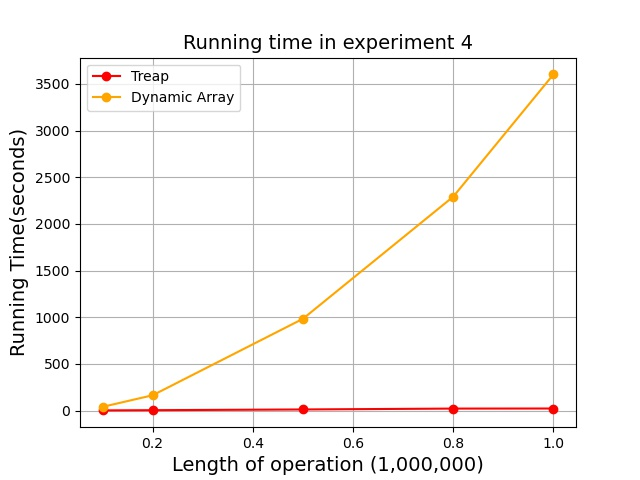
\includegraphics[width=7.5cm]{exp4.jpg} %[pic size]{pic path}
\caption{Running time for different size of mixed operations}\label{figure4} %pic title
\end{figure}

The running time is shown in Figure \ref{figure4}.
The line of treap keeps in the bottom of the figure, because all three operations have the same complexity of time, the $O(log\ n)$.
Thus the increasing of the line will be very small.
Different from treap, the dynamic array has a complexity of $O(1)$ for insertion and $O(n)$ for search and deletion.
The line of dynamic array in Figure \ref{figure4} is a combination of complexities above and becomes a concave up curve.

\section{Conclusion}
The experiments above have identified the different performances between treap and dynamic array.
Because of different data structures, dynamic array has less running time than treap in insert operation, 
meanwhile treap will run faster than dynamic array in search and delete operations, especially when the size of data comes to around 1,000,000.
In practice, treap and dynamic array will not perform very differently on small data.
However, on big data, dynamic array will play well when more insertions, less searches and deletion are needed.
Otherwise, treap will be more efficient.

\nocite{*}
\bibliographystyle{apalike}
% \bibliography{A3}

\end{document}
